\PassOptionsToPackage{unicode=true}{hyperref} % options for packages loaded elsewhere
\PassOptionsToPackage{hyphens}{url}
%
\documentclass[10pt,xcolor=table,color={dvipsnames,usenames},ignorenonframetext,usepdftitle=false,french]{beamer}
\setbeamertemplate{caption}[numbered]
\setbeamertemplate{caption label separator}{: }
\setbeamercolor{caption name}{fg=normal text.fg}
\beamertemplatenavigationsymbolsempty
\usepackage{caption}
\captionsetup{skip=0pt,belowskip=0pt}
%\setlength\abovecaptionskip{-15pt}
\usepackage{lmodern}
\usepackage{amssymb,amsmath,mathtools,multirow}
\usepackage{float,hhline}
\usepackage{tikz}
\usepackage{mathtools}
\usepackage{ifxetex,ifluatex}
\usepackage{fixltx2e} % provides \textsubscript
\ifnum 0\ifxetex 1\fi\ifluatex 1\fi=0 % if pdftex
  \usepackage[T1]{fontenc}
  \usepackage[utf8]{inputenc}
  \usepackage{textcomp} % provides euro and other symbols
\else % if luatex or xelatex
  \usepackage{unicode-math}
  \defaultfontfeatures{Ligatures=TeX,Scale=MatchLowercase}
\fi
\usetheme[coding=utf8,language=french,
,titlepagelogo=img/LOGO-ENSAE.png
]{TorinoTh}
% use upquote if available, for straight quotes in verbatim environments
\IfFileExists{upquote.sty}{\usepackage{upquote}}{}
% use microtype if available
\IfFileExists{microtype.sty}{%
\usepackage[]{microtype}
\UseMicrotypeSet[protrusion]{basicmath} % disable protrusion for tt fonts
}{}
\IfFileExists{parskip.sty}{%
\usepackage{parskip}
}{% else
\setlength{\parindent}{0pt}
\setlength{\parskip}{6pt plus 2pt minus 1pt}
}
\usepackage{hyperref}
\hypersetup{
            pdfborder={0 0 0},
            breaklinks=true}
\urlstyle{same}  % don't use monospace font for urls
\newif\ifbibliography
% Prevent slide breaks in the middle of a paragraph:
\widowpenalties 1 10000
\raggedbottom
\AtBeginPart{
  \let\insertpartnumber\relax
  \let\partname\relax
  \frame{\partpage}
}
\setlength{\emergencystretch}{3em}  % prevent overfull lines
\providecommand{\tightlist}{%
  %\setlength{\itemsep}{0pt}
  \setlength{\parskip}{0pt}
  }
\setcounter{secnumdepth}{0}

% set default figure placement to htbp
\makeatletter
\def\fps@figure{htbp}
\makeatother

\usepackage{bclogo}
\usepackage{cancel}
\usepackage{multirow}
\usepackage{booktabs}
\usepackage{fontawesome5}

\title{Histoire du recensement de la population en France}
\ateneo{Histoire et épistémologie de la statistique}
\author{Kim Antunez \(\qquad \qquad \qquad \qquad\) Romain Lesauvage\\
Alain Quartier-la-Tente}
\date{}


\setrellabel{}

\setcandidatelabel{}

\rel{}
\division{ENSAE 3A}

\departement{(2020-2021)}
\makeatletter
\let\@@magyar@captionfix\relax
\makeatother


\begin{document}
\begin{frame}[plain,noframenumbering]
\titlepage
\end{frame}

\begin{frame}{Retracer cette histoire avec divers supports d'archive}
\protect\hypertarget{retracer-cette-histoire-avec-divers-supports-darchive}{}
\begin{figure}
\begin{picture}(200,150)   
\put(10,-50){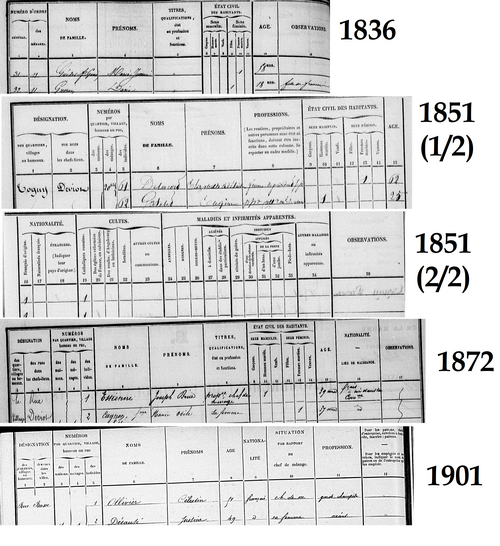
\includegraphics[width=0.6\textwidth,angle=-10,origin=c]{img/support1.png}}
\pause
\put(-60,-50){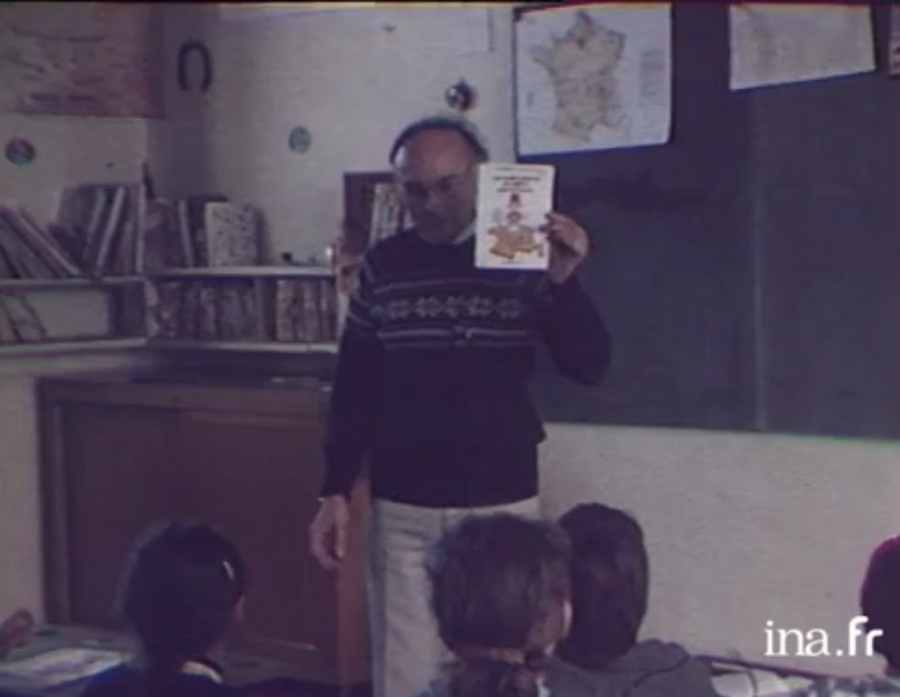
\includegraphics[width=0.8\textwidth,angle=10,origin=c]{img/support2.png}}
\pause
\put(-100,-20){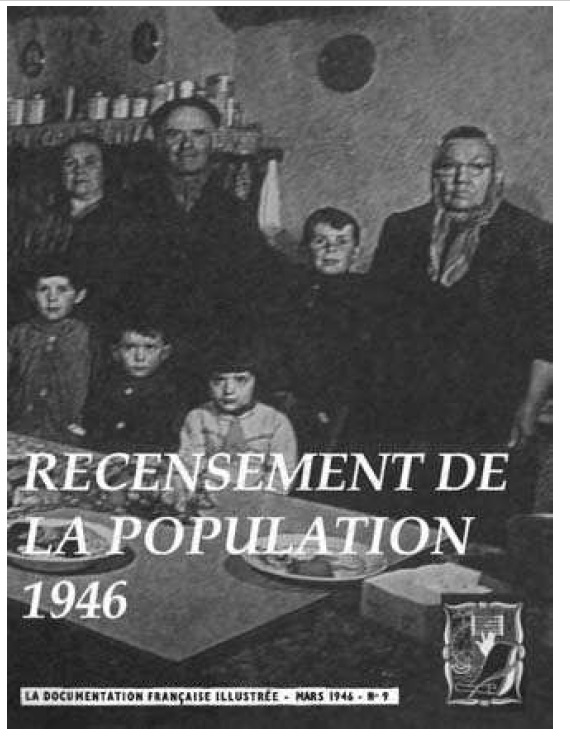
\includegraphics[width=.4\textwidth,angle=-35,origin=c]{img/supporta.jpg}}
\put(20,-30){\includegraphics[width=.4\textwidth,angle=0,page=3]{img/supportb.png}} 
\put(90,-40){
\includegraphics[width=.4\textwidth,angle=45,origin=c, page=2]{img/supportc.jpg}}
\pause
\put(-75,-40){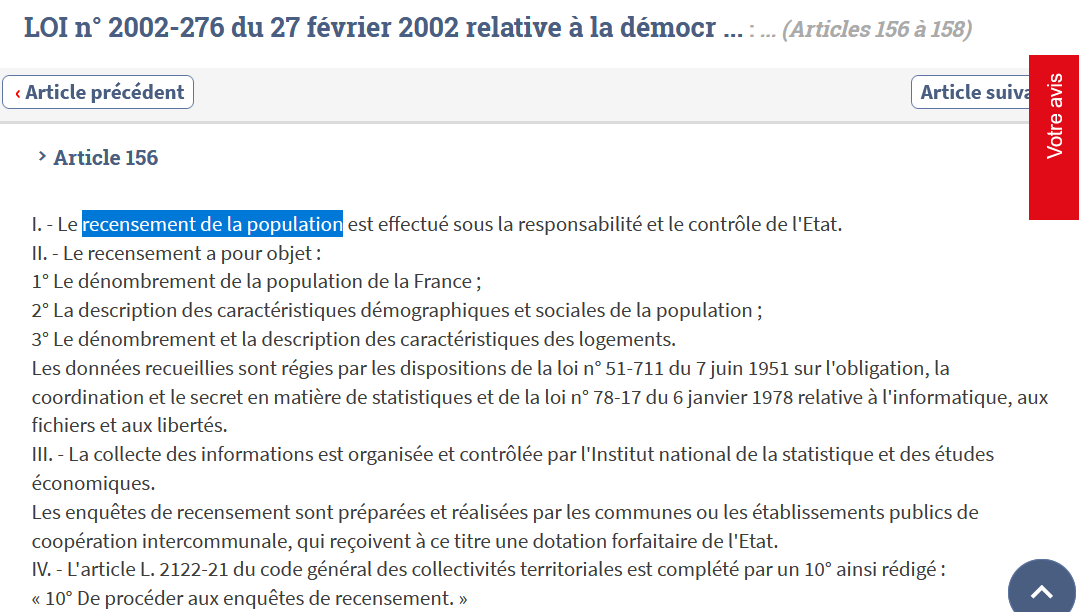
\includegraphics[width=1.1\textwidth,angle=0,origin=c]{img/support3.png}}
\pause
\put(-10,-20){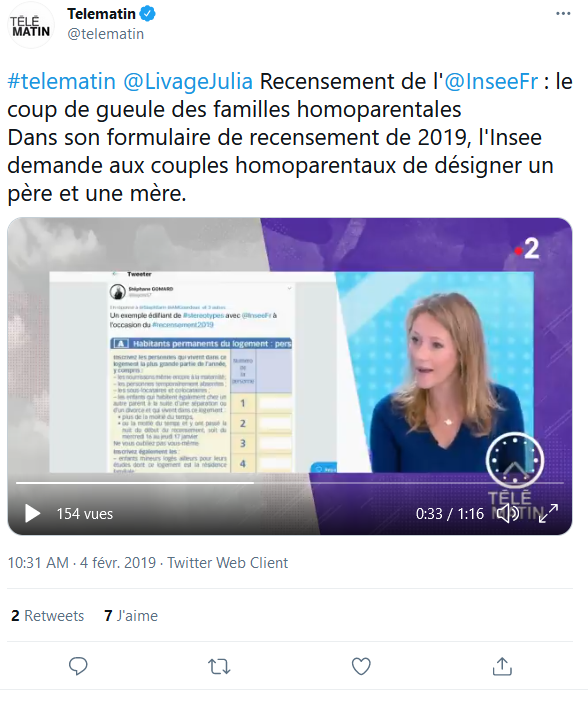
\includegraphics[width=0.6\textwidth,angle=30,origin=c]{img/support4.png}}
\end{picture}    
\end{figure}
\end{frame}

\hypertarget{histoire-du-recensement}{%
\section{Histoire du recensement}\label{histoire-du-recensement}}

\begin{frame}{Sommaire}
\protect\hypertarget{sommaire}{}
\tableofcontents[currentsection, hideothersubsections]
\end{frame}

\begin{frame}{XIVe siècle : Statistique des feux et exigences fiscales}
\protect\hypertarget{xive-siuxe8cle-statistique-des-feux-et-exigences-fiscales}{}
Quelques dates clefs \dots

\begin{itemize}
\item
  \textbf{1er siècle av JC} : Recensement de 368 000 habitants d'un camp
  helvète (\emph{Jules César})
\item
  \textbf{786} : Recensement des sujets de plus de 12 ans astreints à
  prêter serment (\emph{Charlemagne})
\item
  \textbf{1328} : « Etat des paroisses et feux de bailliages et
  sénéchaussées de France » (\emph{Philippe IV le Valois})
\item
  \textbf{1539} : registres paroissiaux rendus obligatoires, ordonnance
  de Villers-Cotterêts (\emph{François 1er})
\item
  \textbf{1686} : Vauban publie « Méthode générale et facile pour faire
  le dénombrement des peuples » (\emph{Louis XIV})
\end{itemize}
\end{frame}

\begin{frame}{1801 : date du premier recensement français}
\protect\hypertarget{date-du-premier-recensement-franuxe7ais}{}
\bigskip

\begin{figure}
  \caption{Premières lignes de listes nominatives de quelques recensements ayant eu lieu à Togny-aux-Boeufs (département de la Marne) entre 1836 et 1901.}
\begin{center}
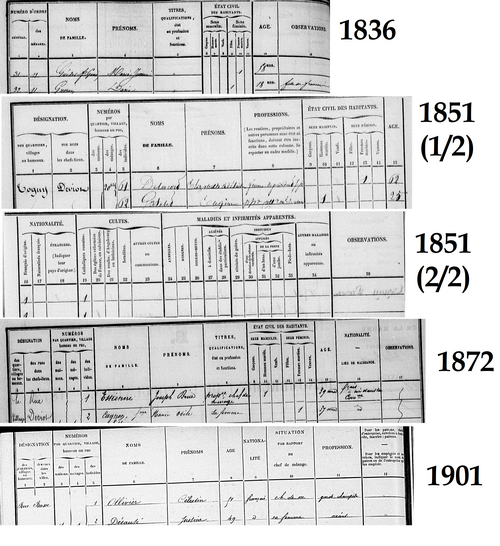
\includegraphics[width = 0.5\linewidth]{img/support1.png}
\end{center}
%\vspace{0.1cm}
\footnotesize
\emph{Source -- archives départementales de la Marne.}
\end{figure}
\end{frame}

\begin{frame}{1946 : prise en charge du recensement par l'Insee}
\protect\hypertarget{prise-en-charge-du-recensement-par-linsee}{}
\medskip

\begin{figure}
  \caption{Schéma de codage informatique de la catégorie de migrant dans le recensement de 1962.}
\begin{center}
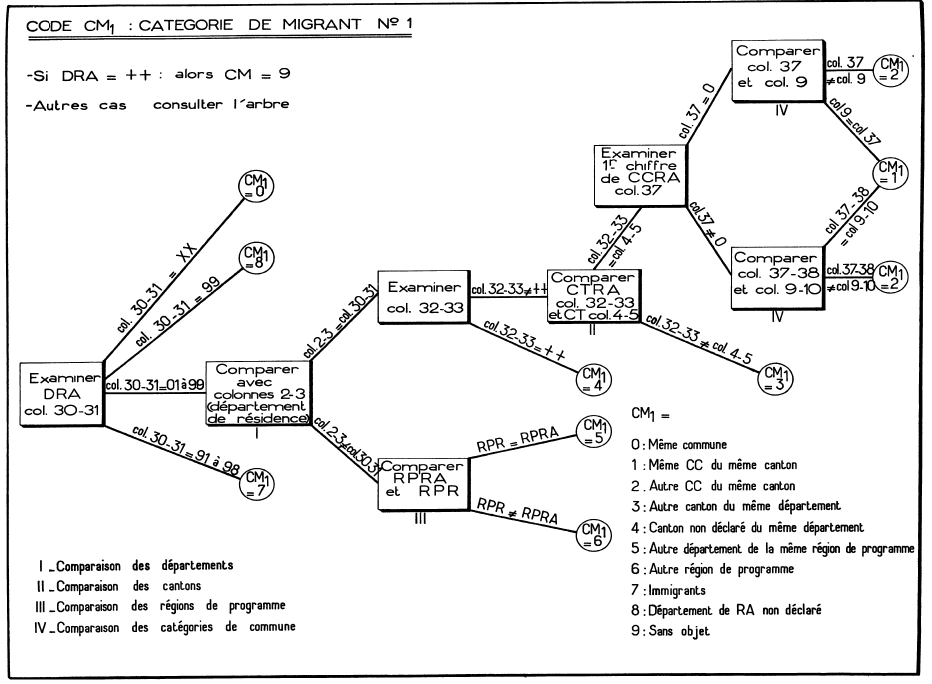
\includegraphics[width = 0.6\linewidth]{img/informatique.png}
\end{center}
%\vspace{0.1cm}
\footnotesize
\emph{Source -- Chevry, 1963.\\Note -- Après un maximum de 6 lectures et comparaisons, l’ordinateur détermine la catégorie de migrant de l’individu et la chiffre sur une bande magnétique.}
\end{figure}
\end{frame}

\hypertarget{focus-sur-la-ruxe9novation-du-recensement-en-2004}{%
\section{Focus sur la rénovation du recensement en
2004}\label{focus-sur-la-ruxe9novation-du-recensement-en-2004}}

\begin{frame}{Sommaire}
\protect\hypertarget{sommaire-1}{}
\tableofcontents[currentsection, hideothersubsections]
\end{frame}

\hypertarget{nouveau-recensement}{%
\subsection{Nouveau recensement}\label{nouveau-recensement}}

\begin{frame}{\bccalendrier 2004 : un nouveau recensement est né}
\protect\hypertarget{un-nouveau-recensement-est-nuxe9}{}
\bclampe Loi de démocratie de proximité du 27 février 2002 : le
recensement est rénové

\textbf{Objectifs :}

\begin{itemize}

\item données plus fraiches

\item lissage des dépenses publiques

%\item améliorations méthodologiques
\end{itemize}

\bigskip

\begin{columns}[T]
\begin{column}{0.48\textwidth}
\highlightbf{Avant (<1999)}

\begin{itemize}
\item recensement exhaustif (tous les 6 à 9 ans)

\smallskip
\item coût ponctuel 150 millions €
\end{itemize}
\end{column}

\begin{column}{0.48\textwidth}
\highlightbf{Après (>2004)}

\begin{itemize}
\item recensement annuel par sondage $\phantom{text{blablabla}}$

\smallskip
\item coût annuel : 30 millions €

%\item méthodes de redressement
\end{itemize}
\end{column}
\end{columns}
\end{frame}

\begin{frame}{Introduction d'un cycle de 5 années}
\protect\hypertarget{introduction-dun-cycle-de-5-annuxe9es}{}
\begin{enumerate}
\item
  Communes de moins de 10 000 habitants :

  \begin{itemize}
  \item
    5 groupes de rotation (représentativité régionale)
  \item
    recensement \highlight{exhaustif} d'1 groupe par an
  \end{itemize}
\end{enumerate}

\medskip 

\begin{enumerate}
\setcounter{enumi}{1}
\item
  Communes de plus de 10 000 habitants :

  \begin{itemize}
  \item
    recensement annuel par \highlight{sondage}
  \item
    RIL : 5 groupes d'adresses (20 \% des logements, représentatitivé de
    la commune)
  \item
    1 groupe enquêté par an avec un tirage de 40 \% des adresses
  \end{itemize}
\end{enumerate}

Pourquoi 10 000 \bcquestion 50 \% de la population française habite dans
des communes de moins de 10 000 habitants
\end{frame}

\hypertarget{des-attentes-et-des-craintes}{%
\subsection{Des attentes et des
craintes\ldots{}}\label{des-attentes-et-des-craintes}}

\begin{frame}{Une meilleure connaissance de la population ?}
\protect\hypertarget{une-meilleure-connaissance-de-la-population}{}
\textit{La théorie...}

\faPlusSquare{} Des données plus fraîches.

\faPlusSquare{} Un meilleur suivi des flux.

\begin{center}\end{center}

\textit{... vs la pratique}

\faPlusSquare{} Une population légale de référence publiée chaque année
\(N\)\ldots{}

\faMinusSquare{} \ldots{} mais datée de \(N-3\).

\faPlusSquare{} Analyse améliorée des mobilités.

\faMinusSquare{} Biais : doubles comptes, conjoncture
\end{frame}

\begin{frame}{Des élus inquiets face à la surcharge de travail}
\protect\hypertarget{des-uxe9lus-inquiets-face-uxe0-la-surcharge-de-travail}{}
\begin{center}\bcattention \end{center}

\faQuestionCircle{} Maires : surcharge de travail, transfert de
compétences de l'État aux communes.

\faQuestionCircle{} Parlementaires : 350 textes juridiques basés sur le
recensement.

\begin{center}\bcsmmh\end{center}

\faMinusCircle{} Mise à jour du RIL compliquée pour les communes.

\faMinusCircle{} Mairies responsables du recensement : agents recenseurs
à recruter, collecte, qualité des adresses.

\begin{center}\bcsmbh\end{center}

\faPlusCircle{} Professionnalisation des équipes en charge du
recensement.
\end{frame}

\begin{frame}{Une précision en péril ?}
\protect\hypertarget{une-pruxe9cision-en-puxe9ril}{}
\begin{center}\bcattention \end{center}

\faQuestionCircle{} Population méfiante face aux sondages.

\faQuestionCircle{} Universitaires inquiets sur la précision.

\begin{center}\bcsmmh\end{center}

\faMinusCircle{} Taux de non-réponse en hausse (3 \% vs 1 \%)

\begin{center}\bcsmbh\end{center}

\faPlusCircle{} Précision toujours élevée : 0,02 \% d'erreur au niveau
national
\end{frame}

\begin{frame}{Conclusion}
\protect\hypertarget{conclusion}{}
\begin{center}\bcoeil\end{center}

Histoire du recensement en France grâce aux archives\ldots{}

\begin{center}\bcstop\end{center}

En 2002 : rénovation, introduction de \highlight{sondages}.

\begin{center}\bcattention\end{center}

Des craintes et doutes\ldots{} mais une précision élevée, baisse de
coûts, fraîcheur des données !
\end{frame}

\begin{frame}[noframenumbering]{Merci pour votre attention !}
\protect\hypertarget{merci-pour-votre-attention}{}
\bigskip

\begin{center}

\includegraphics[width = 3cm]{img/LOGO-ENSAE.png}
\end{center}
\end{frame}

\end{document}
